%-----------------------------------------------------------------------------%
\chapter{ANALISIS DAN PERANCANGAN SISTEM}
%-----------------------------------------------------------------------------%

%
\vspace{4.5pt}

\noindent Bab ini memaparkan analisis masalah yang diatasi berserta pendekatan dan alur kerja dari perangkat lunak yang dikembangkan, mengimplementasikan metode yang digunakan dan hasil yang akan ditampilkan.
\\
\section{Analisis Masalah}
\noindent Pada bab 1 telah dijelaskan bahwa penelitian mengenai sistem pengenalan plat nomor kendaraan merupakan bidang yang masih berkembang dan implementasinya memegang peranan penting dalam bidang transportasi. Pada penelitian ini, penulis menggunakan metode \textit{Canny Detector} dan \textit{Hough Transform} untuk mendeteksi lokasi plat kendaraan, kemudian menggunakan metode \textit{Histogram of Oriented Gradient} untuk mengekstraksi fitur dari citra karakter dari plat nomor yang sudah disegmentasi dengan menghitung grafik horizontal pita, kemudian dilakukan klasifikasi dengan menggunakan metode \textit{Support Vector Machine}.
%\noindent Pada bab 1 telah dijelaskan bahwa mendeteksi manusia merupakan bidang yang masih berkembang dan implementasinya sangat dibutuhkan di berbagai bidang. Pada penelitian ini, penulis menggunakan citra RGB-D agar tetap memiliki hasil yang baik pada kondisi pencahayaan yang relatif gelap. Dengan menggunakan citra kedalaman akan sangat membantu dalam proses deteksi manusia dalam tahap awal, \textit{training}, ataupun tahap \textit{testing}. Penerapan \textit{Convolutional Neural Network} untuk mendeteksi manusia dan Kalman \textit{filter} untuk melacak manusia yang telah terdeteksi. Bagian tubuh manusia yang akan dideteksi adalah bagian tubuh atas sehingga tetap dapat mendeteksi manusia bila terdapat citra manusia yang tertutup atau hanya tampak sebagian.

\noindent Masukan untuk sistem deteksi dan pengenalan plat nomor kendaraan ini adalah citra yang ditangkap oleh kamera DSLR Canon EOS 500 D dan Canon EOS 550 D beresolusi 15 dan 18 megapiksel. Citra tangkapan kemudian akan diubah resolusinya menjadi 1024 $\times$ 640 piksel. Setiap citra masukan berisi bagian depan dari kendaraan yang memiliki plat nomor kendaraan.

\noindent Keluaran atau hasil dari sistem akan berupa teks hasil dari pengenalan karakter pada citra plat nomor kendaraan masukkan.\\ 

\section{Kerangka Pemikiran}
\noindent Berikut ini adalah kerangka pemikiran dari metode yang diusulkan untuk melakukan deteksi plat nomor kendaraan dan melakukan pengenalan karakter pada citra karakter yang terdapat pada plat nomor.\\

\begin{adjustbox}{width=1\textwidth}
	\noindent\begin{minipage}{\linewidth}
	\framebox[\textwidth]{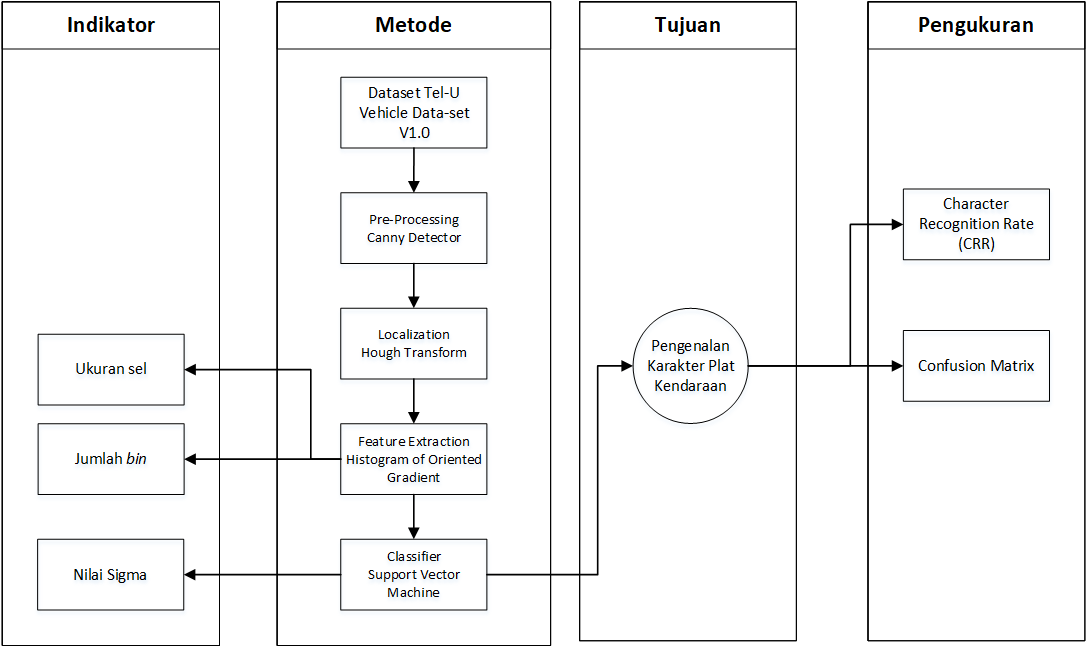
\includegraphics[width=13cm]{images/KerangkaPemikiran.png}}
	\captionof{figure}{Kerangka Pemikiran}
	\label{fig:KerangkaPemikiran}
\end{minipage}
\end{adjustbox}

\noindent Seperti pada gambar \ref{fig:KerangkaPemikiran}, terdapat beberapa variabel indikator yang memengaruhi hasil dan perlu dilakukan penyesuaian, seperti ukuran sel pada metode \textit{Histogram of Oriented Gradient}, jumlah \textit{bin} yang menentukan batasan sudut yang digunakan, dan jumlah data \textit{training} untuk \textit{classifier} \textit{Support Vector Machine}. Penelitian ini memiliki dua tujuan, yaitu untuk melihat hasil akurasi deteksi plat nomor dan akurasi pengenalan karakter pada plat nomor dengan menggunakan \textit{confusion matrix}.\\

\section{Analisis Urutan Proses Global}
\noindent Dalam sistem pengenalan plat nomor kendaraan terbagi atas dua proses yaitu proses \textit{training} dan proses \textit{testing}. Proses \textit{training} dilakukan untuk mendapatkan kelas-kelas dari karakter-karakter yang akan dikenali. Proses \textit{testing} dilakukan untuk menghitung hasil yang berupa akurasi dari pengenalan karakter pada plat nomor kendaraan.\\

\subsection{Proses \textit{Training}}

\begin{adjustbox}{width=1\textwidth}
	\noindent\begin{minipage}{\linewidth}
		\framebox[\textwidth]{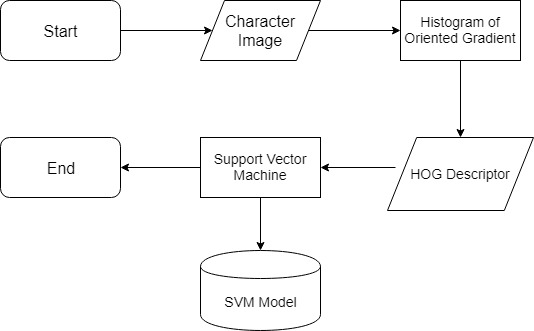
\includegraphics[width=12cm]{images/FlowchartTraining.jpg}}
		\captionof{figure}{\textit{Flowchart Training} Sistem Pengenalan Plat Nomor Kendaraan\\}
		\label{fig:FlowchartTraining}
	\end{minipage}
\end{adjustbox}

Berikut ini adalah uraian dari \textit{flowchart} pada gambar \ref{fig:FlowchartTraining} yang dilakukan dalam penelitian ini:
\begin{enumerate}
\item Citra yang menjadi masukan yaitu dari \textit{dataset English Font} yang berasal dari \textit{The Chars 74K image dataset} yang berisi kumpulan jenis karakter dari komputer dengan 4 variasi, yaitu citra karakter miring (\textit{Italic}), citra karakter tebal (\textbf{Bold}), dan citra karakter normal. Citra karakter memiliki ukuran 128 $\times$ 128 piksel. Citra karakter berwarna hitam dengan latar belakang berwarna putih. Kumpulan karakter yang digunakan adalah karakter angka dari 0 sampai dengan 9 dan karakter huruf kapital dari A sampai dengan Z, karakter huruf kecil tidak digunakan karena pada plat nomor kendaraan tidak menggunakan karakter huruf kecil.
\item \textit{Histogram of Oriented Gradient} berfungsi untuk mendapatkan fitur dari dari citra masukan. Hasil dari ekstraksi fitur dengan menggunakan HOG adalah \textit{HOG descriptor}, yang mendeskripsikan distribusi dari gradien berarah pada suatu area citra.
\item Ukuran sel dan blok yang digunakan untuk proses ekstraksi fitur dengan menggunakan \textit{HOG} adalah 8 $\times$ 8 piksel untuk ukuran sel dan 4 $\times$ 4 sel dan jumlah \textit{bin} yang digunakan pada tahap pembuatan \textit{histogram} adalah 9 dimulai dari 0 derajat hingga 180 derajat.
\item \textit{Support Vector Machine} (SVM) digunakan untuk mengklasifikasikan fitur-fitur yang sudah didapatkan ke dalam kelas-kelas dari karakter yang akan dikenali. Hasil dari klasifikasi ini nantinya akan disimpan ke dalam bentuk berkas.\\
\end{enumerate}

%\begin{spacing}{1}
%\noindent\rule{\textwidth}{1.5pt}
%\textbf{Algoritme \textit{Convolutional Neural Network} tahap %\textit{Training}}
%\begin{enumerate}
%\item Masukkan citra kedalaman yang telah melewati tahap %\textit{pre-processing}.
%\item Inisialisasi nilai setiap \textit{neuron}/\textit{filter}, \textit{learning rate}, dan \textit{epoch}.
%\item Lakukan proses konvolusi (perkalian citra masukan dengan \textit{neuron}), didapatkan \textit{induced local field} dengan persamaan \ref{eq:InducedLocalField}.
%\item Gunakan fungsi aktivasi \textit{rectified linear units} (ReLUs) menggunakan persamaan \ref{eq:RELU}.
%\item Lakukan proses \textit{subsampling} dengan \textit{max pooling} dari nilai pada lapisan sebelumnya. Catat juga indeks yang menyimpan nilai maksimal.
%\item Lakukan proses konvolusi (perkalian masukan dengan \textit{neuron}), didapatkan \textit{induced local field} dengan persamaan \ref{eq:InducedLocalField}.
%\item Gunakan fungsi aktivasi \textit{rectified linear units} (ReLUs) menggunakan persamaan \ref{eq:RELU}.
%\item Lakukan proses \textit{subsampling} dengan \textit{max pooling} dari nilai pada lapisan sebelumnya. Catat juga indeks yang menyimpan nilai maksimal.
%\item Pada lapisan \textit{fully connected}, ubah masukan menjadi vektor (matriks 1 dimensi).
%\item Kalkulasi vektor dengan \textit{filter} dari setiap jenis objek.
%\item Kalkulasi dengan \textit{softmax} menggunakan persamaan \ref{eq:Softmax}, sehingga didapatkan besar probabilitas jenis objek.
%\item Kalkulasi nilai \textit{error} dengan \textit{loss function} \textit{cross-entropy} menggunakan persamaan \ref{eq:crossEntropy}.
%\item Kalkulasi nilai gradien pada setiap lapisan secara terbalik atau mundur.
%\item Kalkulasi ulang nilai pada \textit{neuron} yaitu \textit{weight}/\textit{parameter} sesuai dengan nilai gradiennya masing-masing.
%\item Ulangi langkah 3-14 hingga mencapai \textit{epoch} yang ditentukan.
%\item Simpan model CNN yang berisi \textit{descriptor} CNN beserta nilai \textit{neuron} untuk digunakan pada tahap \textit{testing}.
%\end{enumerate}
%\noindent\rule{\textwidth}{1pt}
%\end{spacing}

%\noindent Dengan \textit{hyperparameter} yang digunakan pada algoritme \textit{Convolutional Neural Network} adalah sebagai berikut:
%\begin{enumerate}
%\item Ukuran \textit{padding} pada seluruh lapisan adalah 0.
%\item Inisialisasi seluruh nilai \textit{kernel} pada lapisan \textit{convolution} dan \textit{fully connected} adalah nilai acak dengan rentang nilai antara -0.005 hingga 0.005.
%\item Inisialisasi seluruh nilai \textit{bias} pada lapisan \textit{convolution} dan \textit{fully connected} bernilai 0.
%\item Pada lapisan \textit{convolution}, ukuran \textit{filter} adalah 5 $\times$ 5 dan \textit{stride} adalah 1.
%\item Pada lapisan \textit{subsampling}, ukuran \textit{kernel} 2 $\times$ 2 dan \textit{stride} adalah 2.
%\item Pada lapisan \textit{fully connected}, ukuran \textit{filter} adalah 1 $\times$ 117, yaitu hasil dari vektorisasi menjadi 1 dimensi dari ukuran 9 $\times$ 13.
%\end{enumerate}

%\begin{spacing}{1}
%\noindent\rule{\textwidth}{1.5pt}
%\textbf{Algoritme \textit{Backpropagation Convolutional Neural Network}}
%\begin{enumerate}
%\item Kalkulasi nilai gradien lokal dari hasil \textit{softmax} dengan persamaan \ref{eq:localGradientOutputSoftmax}.
%\item Kalkulasi nilai gradien lokal, gradien kernel, dan gradien bias pada lapisan \textit{fully connected} dengan persamaan \ref{eq:localGradientOutput} dan hasil dari nilai gradien \textit{softmax} sebelumnya.
%\item Kalkulasi nilai gradien lokal pada lapisan \textit{subsampling} dengan persamaan \ref{eq:localGradientPooling}. Nilai yang teruskan adalah nilai gradien lokal yang merupakan indeks maksimal yang telah dicatat sebelumnya saat proses \textit{forward propagation}.
%\item Kalkulasi nilai gradien lokal, gradien kernel, dan gradien bias pada lapisan \textit{convolution} dengan persamaan \ref{eq:localGradientHidden} dan persamaan \ref{eq:derivativeReLU} sebagai turunan fungsi aktivasi ReLU.
%\item Kalkulasi nilai gradien lokal pada lapisan \textit{subsampling} dengan persamaan \ref{eq:localGradientPooling}. Nilai yang teruskan adalah nilai gradien lokal yang merupakan indeks maksimal yang telah dicatat sebelumnya saat proses \textit{forward propagation}.
%\item Kalkulasi nilai gradien lokal, gradien kernel, dan gradien bias pada lapisan \textit{convolution} dengan persamaan \ref{eq:localGradientHidden} dan persamaan \ref{eq:derivativeReLU} sebagai turunan fungsi aktivasi ReLU.
%\item Perbarui nilai \textit{weight} and bias dengan persamaan \ref{eq:weightCorrection} sesuai dengan nilai gradien lokal yang telah dikalkulasi pada setiap lapisan (seluruh lapisan jenis \textit{convolution} dan \textit{fully connected}).
%\end{enumerate}
%\noindent\rule{\textwidth}{1pt}
%\end{spacing}

\subsection{Proses \textit{Testing}}

\begin{adjustbox}{width=1\textwidth}
	\noindent\begin{minipage}{\linewidth}
		\framebox[\textwidth]{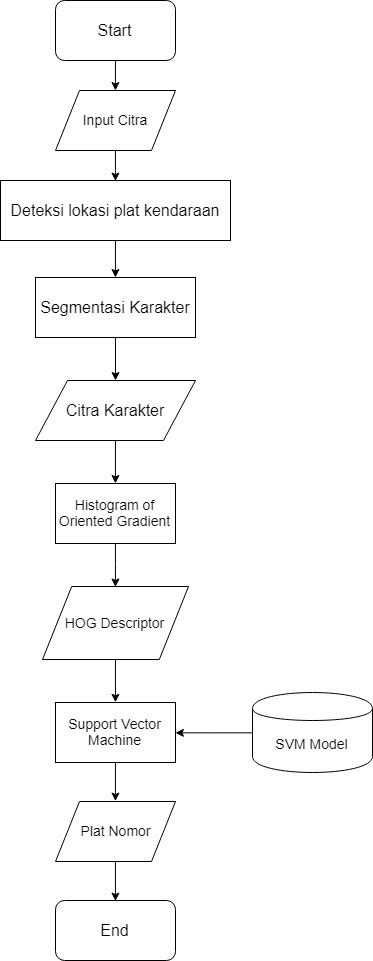
\includegraphics[width=8cm]{images/FlowchartTesting.jpg}}
		\captionof{figure}{\textit{Flowchart Testing} Sistem Pendeteksi dan Pelacakan Manusia\\}
		\label{fig:FlowchartTesting}
	\end{minipage}
\end{adjustbox}

\noindent Pada gambar \ref{fig:FlowchartTesting} terlihat urutan proses \textit{testing}. Pada proses \textit{testing} terdapat beberapa proses yang sama seperti pada proses \textit{training}. Berikut ini adalah uraian dari \textit{flowchart} pada gambar \ref{fig:FlowchartTesting} yang dilakukan dalam penelitian ini:
\begin{enumerate}
\item Citra pengujian yang digunakan didapatkan dari \textit{dataset} plat nomor kendaraan Universitas Telkom yang bernama \textit{Tel-U Vehicle Data-set V1.0}, penggunaan dari dataset ini sesuai dengan perizinan dari institusi yang bersangkutan.
\item Citra yang akan menjadi input dari \textit{HOG} adalah citra hasil dari segmentasi karakter pada citra plat kendaraan pada tahapan deteksi lokasi plat nomor kendaraan.
\item Ukuran dari sel dan blok yang digunakan untuk proses ekstraksi fitur dengan menggunakan \textit{HOG} adalah sama dengan yang digunakan ketika pada tahap \textit{training}.
\item Pada tahap \textit{testing} model SVM yang digunakan diambil dari berkas yang merupakan hasil keluaran dari SVM pada tahap \textit{training}.
\item Hasil keluaran akan berupa sebuah \textit{string} yang menunjukkan kumpulan karakter yang berhasil dikenali oleh sistem.\\
\end{enumerate}

%\begin{spacing}{1}
%\noindent\rule{\textwidth}{1.5pt}
%\textbf{Algoritme \textit{Convolutional Neural Network} tahap \textit{Testing}}
%\begin{enumerate}
%\item Masukkan citra kedalaman yang merupakan kandidat manusia yang telah melewati tahap \textit{pre-processing}.
%\item Muat dan gunakan model CNN dari tahap \textit{training}.
%\item Kalkulasi citra masukan menggunakan model belajar CNN sebelumnya.
%\item Hitung hasil probabilitas dari citra masukan.
%\end{enumerate}
%\noindent\rule{\textwidth}{1pt}\\
%\end{spacing}

%\begin{spacing}{1}
%\noindent\rule{\textwidth}{1.5pt}
%\textbf{Algoritme Kalman \textit{Filter} tahap \textit{Testing}}\\
%\noindent Untuk setiap nilai $x_{1}$, $y_{1}$, $x_{2}$, dan $y_{2}$, lakukan prosedur berikut secara terpisah:
%\begin{enumerate}
%\item Inisialisasi nilai \textit{bounding box} awal, \textit{covariance error} ($P_{k}$), \textit{noise} ($R_{k}$) awal.
%\item Lakukan pembaruan informasi pada iterasi awal untuk adaptasi agar \textit{error} lebih rendah, yaitu kalkulasi Kalman \textit{gain}, estimasi baru, \textit{covariance error} baru.
%\item Setelah dilakukan adaptasi, kalkulasi prediksi nilai posisi dan \textit{covariance error}. Hasil prediksi nilai posisi dapat digunakan untuk membentuk \textit{bounding box}.
%\item Perbarui informasi dengan melakukan pembaruan informasi, yaitu kalkulasi Kalman \textit{gain}, estimasi baru, \textit{covariance error} baru.
%\item Ulangi langkah 3-4 hingga mencapai jumlah pengulangan tertentu.
%\item Ulang dari langkah pertama untuk memperbarui kondisi baru.
%\end{enumerate}
%\noindent\rule{\textwidth}{1pt}\\
%\end{spacing}

\section{Analisis Kasus}
\noindent Pada bagian ini dilakukan analisis tahapan proses dengan melakukan perhitungan manual.\\

\subsection{\textit{Dataset}}
\noindent Dari \textit{The Chars 74K image dataset} untuk tahap \textit{training} akan digunakan citra karakter angka dari 0 sampai dengan 9 dan karakter huruf kapital A sampai dengan Z. Terlihat contoh citra karakter yang ditunjukan pada gambar \ref{fig:ContohCitraDatasetPakai} merupakan contoh karakter angka dan huruf kapital yang akan dipakai. Sedangkan pada gambar \ref{fig:ContohCitraDatasetTakPakai}, gambar tersebut menunjukkan contoh citra karakter yang tidak akan dipakai, yaitu citra karakter tipis, miring, dan karakter huruf kecil. Tidak digunakannya karakter-karakter tersebut dikarenakan pada plat nomor Indonesia, karakter yang digunakan hanyalah karakter huruf kapital dan angka dalam bentuk tegak dan tebal.

\begin{adjustbox}{width=1\textwidth}
	\noindent\begin{minipage}{\linewidth}
		\framebox[\textwidth]{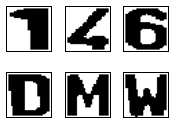
\includegraphics[width=12cm]{images/CitraDatasetPakai.PNG}}
		\captionof{figure}{Contoh citra karakter yang digunakan untuk tahap \textit{training}\\}
		\label{fig:ContohCitraDatasetPakai}
	\end{minipage}
\end{adjustbox}

\begin{adjustbox}{width=1\textwidth}
	\noindent\begin{minipage}{\linewidth}
		\framebox[\textwidth]{
\includegraphics[width=12cm]{images/CitraDatasetTakPakai.PNG}}
		\captionof{figure}{Contoh citra karakter yang tidak digunakan\\}
		\label{fig:ContohCitraDatasetTakPakai}
	\end{minipage}
\end{adjustbox}\\


\subsection{Tahap Pendeteksian Lokasi Plat Nomor}
\noindent Skema alur dari tahap pendeteksian lokasi plat nomor adalah:

\begin{adjustbox}{width=1\textwidth}
	\noindent\begin{minipage}{\linewidth}
		\framebox[\textwidth]{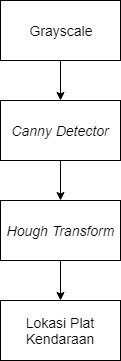
\includegraphics[width=3cm]{images/FlowchartDeteksiPlat.jpg}}
		\captionof{figure}{Skema Alur Pendeteksian Plat\\}
		\label{fig:SkemaAlurPendeteksianPlat}
	\end{minipage}
\end{adjustbox}\\

\subsubsection{\textit{Grayscale}}
\noindent Proses pertama adalah mengubah citra masukan menjadi citra \textit{grayscale}, tujuan dari \textit{grayscaling} citra adalah untuk menghilangkan informasi warna dari setiap piksel citra. Untuk menghitung nilai derajat keabuan setiap piksel, diperoleh dengan rumus:

\begin{table}[H]
	\begin{adjustbox}{width=1\textwidth}
		\begin{tabular}{|p{13.55cm}|}
			\hline
			\begin{equation}\nonumber
			\begin{aligned}
			\textit{grayvalue} 	&= 0.299 R + 0.587 G + 0.114 B&& \\
			\end{aligned}
			\end{equation}\\
			\hline
		\end{tabular}
	\end{adjustbox}
\end{table}

\noindent dimana R, G, B adalah nilai \textit{red}, \textit{green}, \textit{blue} dari masing-masing piksel citra.\\

\subsubsection{Deteksi Tepi Canny}
\noindent Pada bagian ini menjelaskan urutan langkah kerja pada proses Deteksi Tepi Canny. Gambar \ref{fig:FlowchartCannyDetector} adalah \textit{flowchart} Deteksi Tepi Canny.

\begin{adjustbox}{width=1\textwidth}
	\noindent\begin{minipage}{\linewidth}
		\framebox[\textwidth]{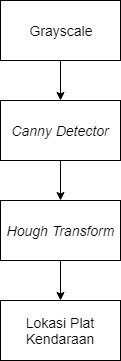
\includegraphics[width=3cm]{images/FlowchartDeteksiPlat.jpg}}
		\captionof{figure}{Flowchart Deteksi Tepi Canny\\}
		\label{fig:FlowchartCannyDetector}
	\end{minipage}
\end{adjustbox}\\

\noindent Hal pertama yang dilakukan untuk deteksi tepi Canny adalah dengan melakukan \textit{smoothing} pada citra dengan menggunakan turunan pertama pertama dari \textit{Gauss} dengan besar \textit{kernel} 3 $\times$ 3 dan nilai dari $\sigma$ = 1 untuk menghilangkan \textit{noise}.

\begin{gather}
\textit{Matriks Gauss Kernel}
=
\begin{bmatrix}
0.077847 & 0.123317 & 0.077847 \\
0.123317 & 0.195346	& 0.123317 \\
0.077847 & 0.123317 & 0.077847
\end{bmatrix}
\label{eq:MatriksGaussKernel}
\end{gather} 

\noindent\textit{Kernel} seperti pada persamaan \ref{eq:MatriksGaussKernel} dikonvolusikan ke dalam citra untuk mendapatkan sebuah nilai baru. Sebagai contoh apabila diambil area pada sebuah citra sebesar 5 $\times$ 5 piksel seperti pada gambar \ref{fig:MatriksCitra} yang kemudian dikonvolusikan menggunakan \textit{kernel} pada persamaan \ref{eq:MatriksGaussKernel}.

\begin{table}[H]
	\centering
	\begin{small}
		\begin{tabular}{|p{1cm}|p{1cm}|p{1cm}|p{1cm}|p{1cm}|}
			\hline
			50 & 50 & 75 & 100 & 100 \\
			\hline
			50 & 50 & 75 & 100 & 100 \\
			\hline
			50 & 50 & 75 & 100 & 100 \\
			\hline
			50 & 50 & 75 & 100 & 100 \\
			\hline
			50 & 50 & 75 & 100 & 100 \\\hline
		\end{tabular}
	\end{small}
	\captionof{figure}{Matriks citra ukuran 5 $\times$ 5\\}
	\label{fig:MatriksCitra}
\end{table}

\noindent Maka pada elemen matriks (2,3) nilainya berubah menjadi:
\begin{table}[H]
	\begin{adjustbox}{width=1\textwidth}
		\begin{tabular}{|p{13.55cm}|}
			\hline
			\begin{equation}\nonumber
			\begin{aligned}
			Matriks[2,3] &= (0.077847 * 50) + (0.123317 * 75) + (0.077847 * 100) \\
						 &+ (0.123317 * 50) + (0.195346 * 75) + (0.123317 * 100) \\
						 &+ (0.077847 * 50) + (0.123317 * 75) + (0.077847 * 100)\\
			\end{aligned}
			\end{equation}\\
			\hline
		\end{tabular}
	\end{adjustbox}
\end{table}

\begin{table}[H]
	\begin{adjustbox}{width=1\textwidth}
		\begin{tabular}{|p{13.55cm}|}
			\hline
			\begin{equation}\nonumber
			\begin{aligned}
			Matriks[2,3] &= 81,166 \approx 81
			\end{aligned}
			\end{equation}\\
			\hline
		\end{tabular}
	\end{adjustbox}
\end{table}

\noindent Sehingga elemen matriks (2,3) berubah nilainya menjadi 81, perhitungan tersebut berlaku untuk semua elemen matriks sisanya, kecuali pada elemen matriks di tepian citra, sehingga seluruh tepian citra sebesar 1 piksel tidak berubah. Berdasarkan perhitungan, maka akan didapatkan hasil matriks citra hasil konvolusi sebagai berikut:

\begin{table}[H]
	\centering
	\begin{small}
		\begin{tabular}{|p{1cm}|p{1cm}|p{1cm}|p{1cm}|p{1cm}|}
			\hline
			50 & 50 & 75 & 100 & 100 \\
			\hline
			50 & 50 & 75 & 100 & 100 \\
			\hline
			50 & 50 & 75 & 100 & 100 \\
			\hline
			50 & 50 & 75 & 100 & 100 \\
			\hline
			50 & 50 & 75 & 100 & 100 \\\hline
		\end{tabular}
	\end{small}
	\captionof{figure}{Matriks citra ukuran 5 $\times$ 5\\}
	\label{fig:MatriksCitra}
\end{table}
%\noindent Tabel \ref{tbl:filteredDataset} merupakan rincian jumlah citra pada masing-masing \textit{dataset} setelah dilakukan pemilihan.
%\begin{table}[H]
%	\centering
%	\begin{small}
%		\captionof{table}{Rincian \textit{Dataset} yang telah dipilih\label{tbl:filteredDataset}}
%		\begin{tabular}{|p{4cm}|p{1cm}|p{3cm}|p{3cm}|}
%			\hline
%			\textbf{Nama \textit{Dataset}} &\textbf{Folder} & \textbf{Jumlah Citra} & \textbf{Jumlah Posisi Manusia}\\
%			\hline
%			\textit{Clothing Store} 			& - & 770 & 1631 \\
%			\hline
%			\multirow{3}{*}\textit{Outdoor}	& 31 & 46 & 218 \\\cline{2-4}
%			& 54 & 84 & 371 \\\cline{2-4}
%			& 56 & 113 & 496 \\\hline
%		\end{tabular}
%	\end{small}
%\end{table}



\newpage